\documentclass[conference]{IEEEtran}
\IEEEoverridecommandlockouts
% The preceding line is only needed to identify funding in the first footnote. If that is unneeded, please comment it out.
\usepackage{cite}
\usepackage{amsmath,amssymb,amsfonts}
\usepackage{algorithmic}
\usepackage{graphicx}
\usepackage{textcomp}
\usepackage{fancyvrb} 
\usepackage{subcaption}
\usepackage{xcolor}
\def\BibTeX{{\rm B\kern-.05em{\sc i\kern-.025em b}\kern-.08em
    T\kern-.1667em\lower.7ex\hbox{E}\kern-.125emX}}
\begin{document}

\title{Performance-portable Parallel Programming in Computer Science Education with Kokkos}

\author{
\IEEEauthorblockN{Jan Ciesko}
\IEEEauthorblockA{\textit{Computer Science Reseach Institute} \\
\textit{Sandia National Laboratories}\\
Albuquerque, NM, USA\\
jciesko@sandia.gov}
\and
\IEEEauthorblockN{David Poliakoff}
\IEEEauthorblockA{\textit{Computer Science Reseach Institute} \\
\textit{Sandia National Laboratories}\\
Albuquerque, NM, USA\\
dzpolia@sandia.gov}
\and
\IEEEauthorblockN{David S. Hollman}
\IEEEauthorblockA{\textit{Computer Science Reseach Institute} \\
\textit{Sandia National Laboratories}\\
Livermore, CA, USA\\
dshallm@sandia.gov}
\and
\IEEEauthorblockN{Christian C. Trott}
\IEEEauthorblockA{\textit{Computer Science Reseach Institute} \\
\textit{Sandia National Laboratories}\\
Albuquerque, NM, USA\\
ctrott@sandia.gov}
\and
\IEEEauthorblockN{Damien Lebrun-Grandié}
\IEEEauthorblockA{\textit{Computational Sciences and Engineering} \\
\textit{Oak Ridge National Laboratory}\\
Oak Ridge, TN, USA\\
lebrungrandt@ornl.gov}
}

\maketitle

\begin{abstract}\label{chap:abstract}
Kokkos is a generic, performance-portable parallel programming model for host- and accelerator architectures in C++. It consists of a pure C++ interface, a specification and a programming library. The programming library exposes patterns and types and maps them to an underlying abstract machine model. 
This machine model offers a generic view of parallel hardware by abstracting from architecture- and vendor-specific programming models. In academia, this can contribute to a generic eduction of performance-portable parallel programming. In this work we present Kokkos from the perspective of educators, highlight key concepts and give an instruction to examples suited for incremental teaching of parallel programming in class.
\end{abstract}
	

%is aligned with C++ standardization efforts and trends towards parallel programming support in base languages. 

\begin{IEEEkeywords}
Parallel programming, accelerator programming, Kokkos, C++
\end{IEEEkeywords}


\section{Introduction}\label{chap:introduction}

Parallel and distributed computing moved into focus at universities and teaching institutions. The interest is two-fold. Firstly, given their role, educators adapt to trends in research and industry and include parallel computing in their curricula, and secondly, parallel computing is an attractive field for department research and industry collaborations. At Sandia, we develop a performance portability library called Kokkos that is ideal for educators looking to teach parallel computing.

In teaching a class on parallel programming, educators must balance considerations of architecture, programming model, and theoretical concepts. Unfortunately, not all architectures support all programming models, nor do many programming models cleanly express all parallel programming constructs. Many vendor models compound this, requiring students have access to specific hardware, and limiting the concepts of parallelism to those supported by that architecture. This makes the choice of programming model important and difficult.

Consequently, generic parallel programming models are needed that target mainstream programming languages and allow a vendor- and architecture independent, performance-portable expression of concurrency. In this way, a parallel program written in a popular language becomes capable of running efficiently on parallel computer architectures that conform to a common parallel machine model specification. We would like to compare this to the support of Von Neumann architectures in programming languages today. We define an abstract machine model later in this work. The lack of such parallel programming models motivated us to develop Kokkos.

Kokkos\footnote{from Greek for grain or seed}~\cite{KOKKOS_PAPER_HERE}, is a performance-portable, parallel programming model for C++ developed at Sandia National Laboratories (SNL) for developing million line scientific software on the world\'s biggest supercomputers. It consists of a programming model specification and a library. The specification defines execution and memory model and an application programming interface (library API). The runtime library exposes functions representing parallel patterns and types for data management and maps them to the underlying abstract execution model. This execution model creates a generic view of compute hardware and memories. The Kokkos library maps execution primitives to vendor-specific programming models, libraries, and memory layouts. Kokkos has been successfully used in many large-scale projects at SNL, LLNL and other research centers~\cite{CITEKOKKOSUSECASES}. Its key properties are

\begin{itemize}
\item Parallel programming model for C++
\item Targets an abstract machine model
\item Implements parallel patterns and tasking paradigms
\item Offers abstract data types for performance portability
\item Pure C++ implementation through template metaprogramming
\item Aligns with C++ standardization efforts for parallel programming
\item Vendor- and architecture independent and open-source
\item Includes exercises and teaching material
\end{itemize}

The objective of this paper is to present Kokkos from two perspectives. Firstly, we would like to present our thoughts that accompanied the design and development of the Kokkos parallel programming model. These insights may be considered useful in parallel programming classes that introduce programming models and reason about design choices.

Further, we would like to present Kokkos to the educational community as one representative parallel programming model for a trend towards architecture-independent and performance-portable programming of CPUs and accelerators. We show an abstraction with enough semantic information to produce performance-portable, parallel code on current architectures. Further, we highlight its alignment and contributions to standardization efforts towards supporting parallel programming in C++. 

Secondly, we would like to promote Kokkos to students and educators as a platform to understand and experiment with parallel patterns in a fashion that is

\begin{itemize}
\item Generic
\item Vendor-agnostic
\item Declarative
\end{itemize}

First, Kokkos has semantics that are generic. This means that students are learning parallelism detached from any architectural concerns. Kokkos won\'t require them to know the specifics of the \"symmetric multiprocessors\" of a GPU or the cache hiearchy on a CPU\footnote{Though nothing precludes an educator from teaching these independently of the model}. Finally, Kokkos is vendor agnostic. If you have a computer lab with processors from one vendor and your students have processors from another, this presents no problem, Kokkos likely works on both. Kokkos is declarative, students aren\'t saying \"map these work items to this set of threads\" but \"do a reduction over this set of data.\" This is critical, much of software engineering is moving to declarative models and languages, learning to operate in such a mindset is useful outside of parallel programming.

The rest of this paper is structured as follows. The next Chapter gives an overview on parallel programming concepts and presents the notion of \emph{semantic capture}. Chapter~\ref{chap:kokkosMM} presents the abstract machine model used to derive required semantic information for performance portability in Kokkos. Chapters~\ref{chap:kokkosPM} and ~\ref{chap:kokkosBackend} present the Kokkos programming model and its back-end support. Chapters~\ref{chap:c++} and~\ref{chap:related} show the alignment to C++ standardization efforts and dicuss related work and lastly Chapter~\ref{chap:conclusion} concludes this work.
           %label: chap:introduction
\section{Towards Generic Parallel Programming}\label{chap:background}

A programming model exposes constrained semantics that the programmer uses to express intent. Absent a programming model providing additional constraints, the semantics of C-like languages can lead to sequential thinking and execution. Parallel programming models expose parallel semantics to enable developers to add concurrency to their code. This is commonly achieved by adding annotations to the base programming language, often through \emph{pragma} clauses or similar language extensions. Other methods expose such semantics through library calls or new languages. All three approaches are conceptually suitable to represent programming paradigms such as tasking, data parallelism, and other patterns. Some representatives are the OpenMP programming model~\cite{OPENMP}, threading libraries, or languages like Erlang\cite{ERLANG} in which parallelism is a first-class citizen. In general, it is up to the parallel programming model implementer to expose language constructs or library interfaces (APIs) that combine convenience to the programmer with a sufficiently constrained semantics that is used to map the program execution to the parallel computer hardware efficiently and correctly. Questions of which semantic information is needed, what paradigm to present, and by what syntactic means to do so span an exciting design space that is well worth exploring.

 Figure~\ref{figSemCapture} shows the four properties that constitute a parallel programming model and its design. We call it the semantic capture.

\begin{figure}[h]
\begin{minted}[fontsize=\small]{text}
Constrained Semantics: memory allocations, 
memory movement, execution parameters
Parallel Paradigms: patterns, tasks
Expression: language 
Control Paradigm: prescriptive, descriptive
\end{minted}
\caption{Semantic capture: a set of constrained semantics, parallel paradigms, expression and concern define key properties of a parallel programming model.}
\label{figSemCapture}
\end{figure}

\emph{Constrained Semantics} provided by the programmer to the parallel programming model can be grouped into information to express intent or correctness and properties that control critical performance aspects. They address the question of \emph{what}, \emph{where} and \emph{how}. In the context of parallel programming, these correspond to defining which code portion to parallelize, where to run the code, where to access the data, and how to run that parallel code. Synchronization primitives may be considered part of the \emph{what}, and information on the execution properties such as data placement or memory access type may be considered as part of the \emph{how}. Application logic is expressed following a \emph{paradigm} implemented in a \emph{programming language}.

A \emph{Parallel Paradigm} is an abstract representation to facilitate the programmer's understanding of programming rules and program behavior. Which programming paradigm to choose depends on several considerations. Parallel patterns allow the programmer to permit concurrent execution for commonly occurring programming patterns such as loop constructs. Tasking is a paradigm that supports the expression of interdependent work items needed for irregular algorithms. Distributed and correctness-oriented programming models may implement actor-based programming, where each unit of execution represents an actor who communicates over predefined communication channels. This paradigm eliminates access to a shared state and aligns well with message passing programming (MPI). The execution model and memory model aspects of a programming model define its behavior. That is, it defines the relationship between abstract concepts and program execution on a given hardware architecture.

A language defines the syntax of the parallel semantics. Annotations-based languages add semantic information to the base language through pragmas while embedded programming models rely on the base language and offer additional programming interfaces to capture information. Their semantics is defined in the API specification. 

Lastly, a programming model must divide responsibility between the developer and the model. We refer to this as defining the \emph{Control Paradigm}. In practice, this is a choice between defining a descriptive and prescriptive semantics. Descriptive semantics requires a developer to express intent. The implementation is the responsibility of the programming model and of the underlying toolchain. Prescriptive semantics requires the developer to specify the mechanisms by which their intent will be implemented. In a prescriptive model, developer success is tied to their knowledge of implementation mechanisms. In a descriptive model that success is tied to the developer's ability to accurately describe their requirements and the toolchain's ability to turn that into implementation. 

Figures~\ref{figOMPLike} and~\ref{figKokkosLike} show two code examples using the aforementioned parallel programming syntaxes. While both programming models implement the same programming paradigm (parallel patterns), Figures~\ref{figOMPLike} extends the base programming language through pragma annotations. Both, pragma annotations and an API call as shown in Figure~\ref{figKokkosLike} can have a descriptive or prescriptive semantics of describing a parallel loop construct. It is up to the programming model specification to make further definitions regarding the separation of concern.

Both examples provide the semantic information on what to parallelize, however, they do not expose enough abstraction primitives that would allow them to map parallel execution on modern architectures efficiently. To define what further information is needed to express concurrency on modern computer architectures, it is important to define an~\emph{abstract machine representation} first. In the following chapters we use the words \emph{representation} and \emph{model} interchangeably. In this work, the abstract machine model does not describe a computer in terms of automata theory but in terms of physical or functional components.

\begin{figure}
\begin{minted}[fontsize=\small]{c++}
#pragma model parallel loop
for ( size_t i = 0; i < N; ++i) {
 /* loop body */
}
\end{minted}
\caption{Annotations-based programming models extend the semantic of the base language through pragma annotations.}
\label{figOMPLike}
\end{figure}

\begin{figure}
\begin{minted}[fontsize=\small]{c++}
model::parallel_for (N, [=] ( const size_t i) {
  /* loop body */
});
\end{minted}
\caption{Embedded parallel programming uses the base language and relies on programming interfaces to capture information.}
\label{figKokkosLike}
\end{figure}
     %label: chap:background
\section{The Kokkos Machine Model}\label{chap:kokkosMM}

The Kokkos machine model defines abstractions that represent hardware capabilities for processing and data access. The Kokkos parallel programming model exposes these abstractions to the programmer through C++ and the Kokkos API. By abstracting from physical hardware, the machine model ensures that applications written in programming models targeting this machine model are generic and performance-portable on current and future hardware. The Kokkos parallel programming model is one particular instance of a programming model that builds on top of that machine model. We would like to point out that it is this conceptual differentiation that allows scenarios where the underlying machine model is instantiated in other languages beyond C++, yet the algorithmic specification as well as performance characteristic and portability remain the same. 

The Kokkos abstract machine representation targets a design of a future shared-memory computing architectures. The design is shown in Figure~\ref{fig:execspace}. It is characterized by multiple latency-optimized execution units and off-die bandwidth-optimized accelerators. Both compute device types can have disjoint memory address spaces with unique performance properties. In such an architecture, execution units might be hierarchically organized with multiple levels of achievable parallelism with different memory access characteristics and coherence properties of caches. In order to ensure performance portability on such a wide range of configurations, an abstraction of compute resources and available memories are required. For this purpose we introduce the abstract concept called \emph{space}.

An instance of an \emph{execution space} is an abstraction over an execution resource to which a programmer can target parallel work. For example, an execution space can be used to describe a multi-core processor. In this case, the execution space contains several homogeneous cores organized into arbitrary logical groups. In a parallel programming model that implements this machine model, an instance of such an execution space would be made available to the programmer to run kernels. Adding more logical groups or accelerators simply increases the number of available execution spaces to the programmer.

Memory and memory types are exposed through \emph{memory spaces}. Each memory space provides storage capacity at which data structures can be allocated and accessed. Different memory space types have different characteristics with respect to accessibility from execution spaces and performance. 

An instance of a memory space provides a concrete method for the application programmer to request data storage allocations. Following the architecture as discussed earlier, the multi-core processor may contain multiple memory spaces that abstract on-package memory, slower DRAM and non-volatile memories. Accelerators can provide an additional memory space through its local on-package memory. An example of such an architectural layout is shown in Figure~\ref{fig:memspace}. The programmer is free to decide where each data structure is allocated by requesting the corresponding memory space. Programmatically this is achieved by instantiating the according memory space. Kokkos provides the appropriate abstraction of memory allocation and data management. We believe that an abstract representation of execution- and memory devices is a key property towards performance-portable parallel programming.

How a machine model is exposed to the programmer and what are the design considerations towards defining an appropriate semantic capture are discussed in the next section.

%Ang, J.A., et. al., Abstract Machine Models and Proxy Architectures for Exascale Computing, 2014, Sandia National Laboratories and Lawrence Berkeley National Laboratory, DOE Computer Architecture Laboratories Project

\begin{figure}
\begin{subfigure}[b]{0.48\textwidth}
\centering
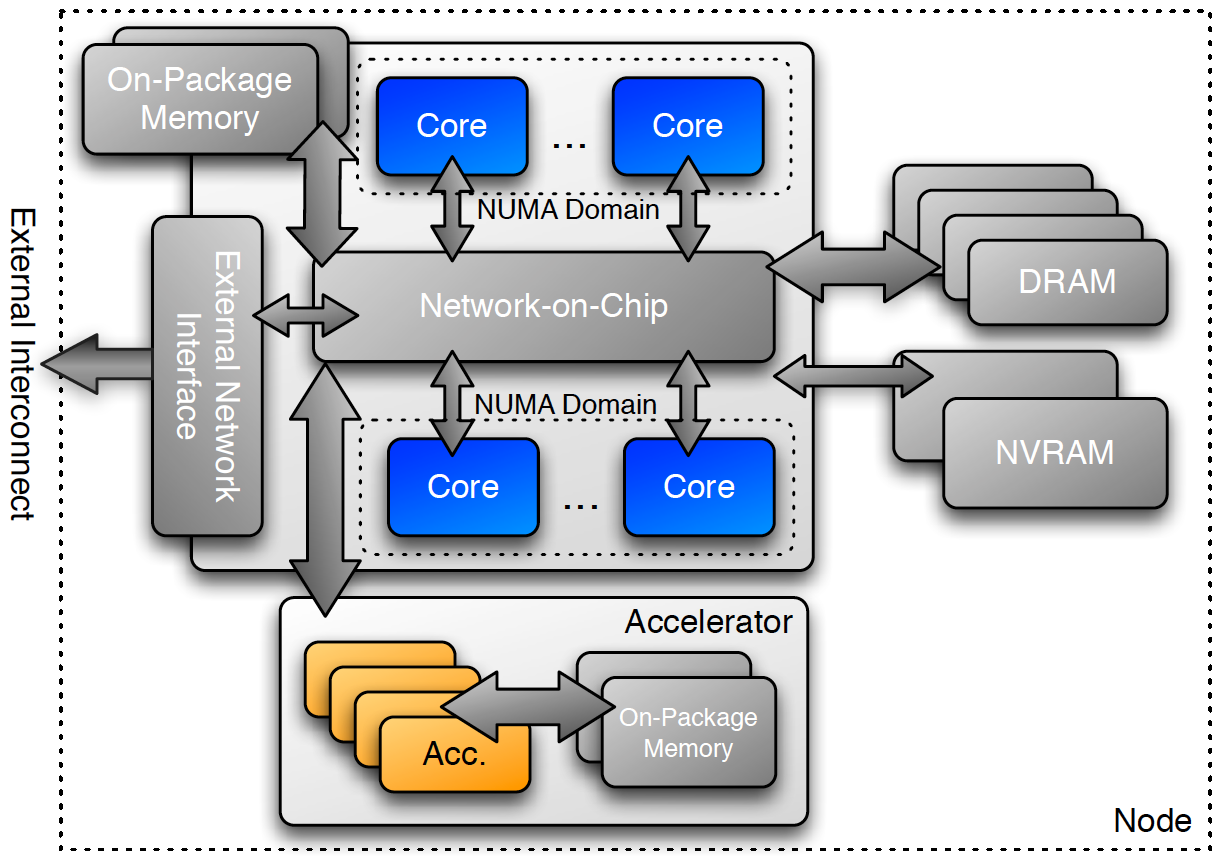
\includegraphics[width=\textwidth]{img/ExecSpaces.png}
\caption{Execution space is an instantiation of a space that represents a processing device to which the programmer can target parallel code.}
\label{fig:execspace}
\end{subfigure}
\hfill \break
\begin{subfigure}[b]{0.48\textwidth}
\centering
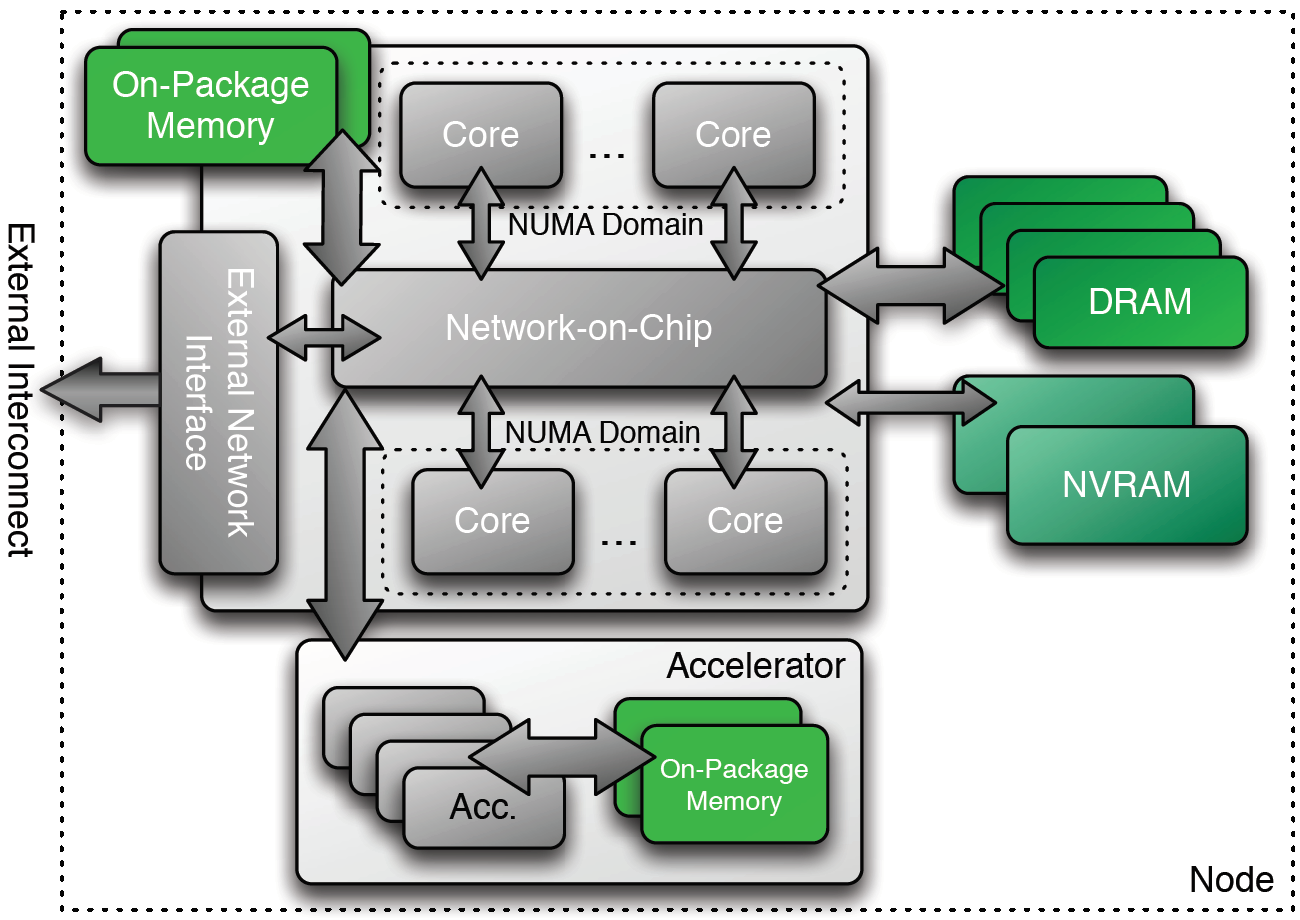
\includegraphics[width=\textwidth]{img/MemSpaces.png}
\caption{A memory space is an instantiation of a space that represents a memory location on which the programmer can allocate data.}
\label{fig:memspace}
\end{subfigure}
\caption{Spaces represent conceptual building blocks of the abstract machine model in Kokkos.}
\label{fig:spaces}
\end{figure}
           %label: chap:kokkosPM
\section{The Kokkos Programming Model}\label{chap:kokkosPM}

The Kokkos programming model specifies a programming paradigm and an API. The API exposes the machine representation to the developer and defines a set of patterns and types that capture intents and properties of execution. This completes the semantic capture, discussed in Chapter~\ref{chap:background}. We detail all three components as follows.

Kokkos defines a pure interface for C++ and uses C++ as a programming language. This has multiple reasons. It is our experience that developers of scientific and high-performance computing applications express the demand for C++ and a generic parallel programming model to support their codes. Further, following their estimates, porting efforts towards adapting to vendors, programming models, APIs, and software releases represent a burden worth addressing. Lastly, the possibility to maintain pure C++ codes is appealing from the code development and debugging perspective. 

From the programming model perspective, C++ offers template metaprogramming which is well suited to implement generic APIs and libraries. In this case, class specialization and templating allow for compile-time generated types and optimizations for a given hardware architecture. 

Using the programming language, a parallel programming paradigm can be applied to simplify the process of thought. Kokkos supports parallel patterns and tasking. Parallel patterns cover \emph{for}, \emph{scan} and \emph{reduction}. This allows the expression of concurrency over iterative, for-loop computable algorithms. To cover the class of while-loop computable algorithms (irregular algorithms), Kokkos implements the tasking paradigm. Tasks encapsulate work into units that may be executed in parallel to other tasks or sections of the program. Equipped with a language and set of paradigms, a particular set of abstractions can be defined to expose the abstract machine model and capture the intent of the programmer.

To capture semantic information, that is the~\emph{what}, the~\emph{where}, and the~\emph{how}, Kokkos introduces six abstractions:~\emph{execution spaces},~\emph{execution patterns},~\emph{execution policies},~\emph{memory spaces},~\emph{memory layout}, and~\emph{memory traits}. These abstractions specify semantic information that enables to capture the programmer's intent and allows the runtime to efficiently map the program to any underlying hardware architecture. We list them as follows:
\begin{itemize}
	\item  An execution space is a place where code can be executed. On current hardware architectures, this corresponds to accelerators and CPUs and can include other compute devices in the future. This abstraction supports remote compute devices in distributed memory scenarios as remote execution spaces.
	\item Execution patterns expose the parallel programming paradigm. Supported patterns are the \emph{parallel\_for} loop that executes the loop body in any order a specified amount of times, the \emph{parallel\_reduce} which combines a parallel\_for with a reduction operation, the \emph{parallel\_scan} which combines a parallel\_for operation with a prefix or postfix scan, and \emph{task} which executes a single function potentially in parallel with respect to other tasks or code sections. 
	\item Execution policies shape the iteration space of a loop pattern. A simple execution policy is a range policy. It specifies that the loop body is executed once for each element in a range.
	\item Memory spaces are the places where data resides. They specify the physical locations of data as well as access characteristics. Different physical locations correspond to different device types such as high bandwidth memories, on-die scratch memories, or non-volatile bulk storage. Different logical memory spaces allow for concepts such as memory in the CUDA programming model, which is accessible from the host and the CUDA accelerator. Memory spaces, similarly to execution spaces, conceptually support remote memory locations in distributed-memory scenarios. Furthermore, they encapsulate functionality such as consistency control and persistence scopes.
	\item Layouts express the mapping from array indices to address offsets. By adopting appropriate layouts for memory structures, an application can optimize data access patterns in a given algorithm. If an implementation provides polymorphic layouts (i.e. a data structure can be instantiated at compile or runtime with different layouts), architecture-dependent optimizations can be performed.
	\item Memory traits specify how a data structure is accessed. Traits express usage scenarios such as atomic access, random access, and streaming loads or stores. This allows the programming model to optimize load and store operations.
\end{itemize}

\begin{figure}[t!]
\begin{minted}[fontsize=\small]{c++}
template <class ExecPolicy, class FunctorType>
Kokkos::parallel_for(const std::string& name, 
 const ExecPolicy& policy, 
 const FunctorType& functor);
\end{minted}
\caption{The Kokkos~\emph{parallel\_for} class shows how template metaprogramming allows to specialize types. Its descriptive semantic offers the freedom to optimize execution on modern architectures with multiple degrees of concurrency where an execution policy (\emph{ExecPolicy}) shapes the iteration space accordingly.}
\label{fig:parallelFor}
\end{figure}

Figure~\ref{fig:parallelFor} shows one definition of the Kokkos~\emph{parallel\_for} interface. This interface accepts two template parameters and three function arguments. \emph{ExecPolicy} shapes the iteration space for a particular execution space. Examples of execution policies are the~\emph{RangePolicy}, ~\emph{MDRangePolicy} and the~\emph{TeamPolicy}. As the name suggests, these policies express iteration spaces. For example, a range policy defines a one-dimensional iteration range. The MDRangePolicy represents a multi-dimensional iteration space and is used to express tightly nested loop patterns. A team policy defines a 1D iteration range, each of which is assigned to a team of threads. This policy allows the expression of hierarchical parallelism. The second template parameter,~\emph{FunctorType}, represent a functor that implements the~\emph{()-operator} with a matching signature for the given execution policy. The functor can be defined using a C++ class, struct or lambda expression. We would like to highlight that the return semantic of the parallel\_for is defined as \emph{potentially asynchronous}. To guarantee a kernel has finished, a developer should call the fence of the execution space on which the kernel is being executed. Otherwise, it depends on the execution space where the loop executes and whether this execution space implements a barrier. 

\begin{figure}[t!]
\begin{minted}[fontsize=\small]{text}
Constrained Semantics: Patterns (intent),
Spaces, Layouts, Policies and Traits
Parallel Paradigms: Parallel patterns and 
tasking
Expression: Embedded, C++
Control Paradigm: descriptive
\end{minted}
\caption{Semantic capture defined by the Kokkos programming model.}
\label{fig:SemCaptureKokkos}
\end{figure}

The semantic of the parallel\_for class in Kokkos demonstrates the descriptive nature of the programming model. Programming with patterns and abstractions allows the compiler to generate optimized transformations. 
Generally, parallel patterns in Kokkos do not guarantee iteration ordering nor the degree of concurrency during their execution. This gives the freedom to the underlying abstraction layers to implement different mapping patterns on different hardware such as the assignment of iterations to threads or vector lanes. We believe that these abstractions and their descriptive semantic represent key programming primitives and the way forward for generic support for parallel programming. In conclusion, Figure~\ref{fig:SemCaptureKokkos} shows the semantic capture defined by the Kokkos programming model. Figure~\ref{fig:abstractions} summarizes patterns and abstractions and structures them by information type in the semantic capture.

To the interested reader, the complete programming model description can be accessed on-line\cite{KOKKOS_WIKI}.
The next section shows an example of the Kokkos parallel\_for and explains how it is mapped to the underlying backend programming model.

\begin{figure}[t!]
\centerline{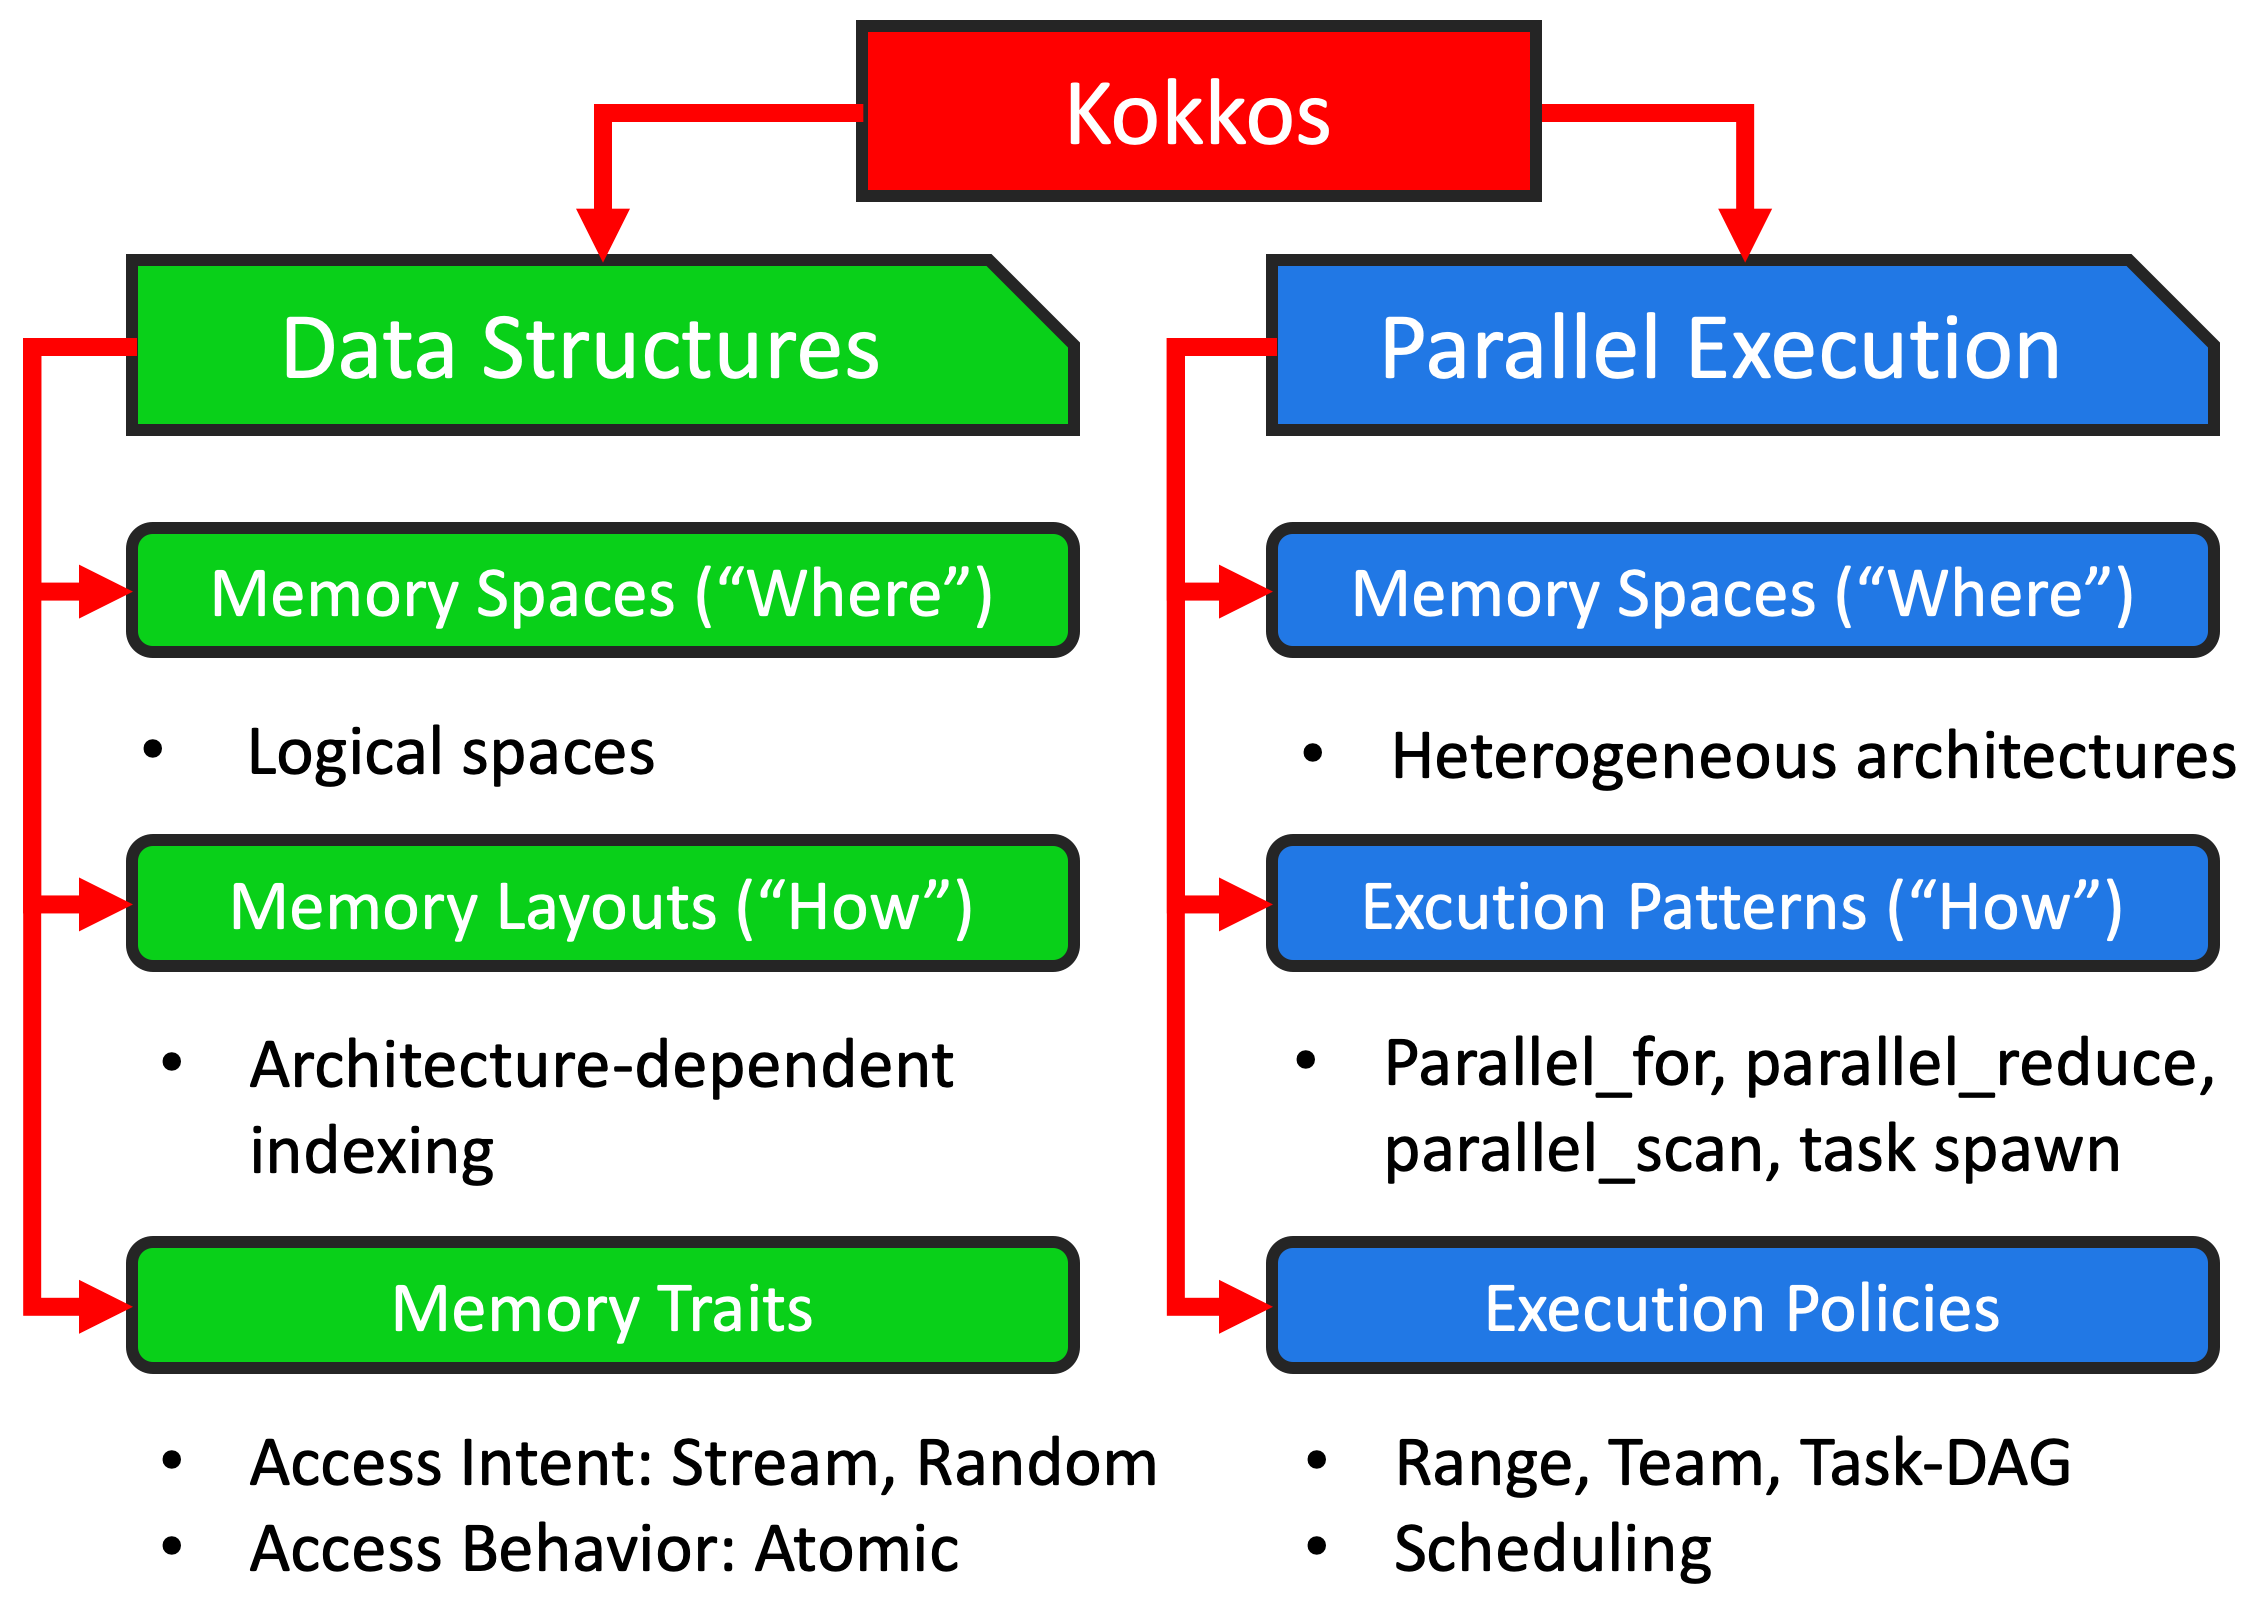
\includegraphics[width=0.49\textwidth]{img/Abstractions.png}}
\caption{Overview of abstractions that define the constrained semantic of the Kokkos parallel programming model.}
\label{fig:abstractions}
\end{figure}
        %label: chap:kokkosEMA
\section{Example}\label{chap:kokkosExample}

This section provides a practical insight into programming with Kokkos and the inner workings of the programming model library. Figure~\ref{fig:KokkosExample} shows am example application that algorithmically initializes an array to integers and includes several points of interests. Taking a closer look, the reader can observe the initialization and finalization of the Kokkos runtime library through the~\emph{Kokkos::initialize} and~\emph{Kokkos::finalize} method calls. Further the example shows the use of the~\emph{view} abstraction that represents a one-dimensional integer array of size~\emph{N}. The object carries the name~\emph{A} internally to facilitate tracing and debugging. In this example, a parallel\_for pattern object receives a range policy that is templated to the OpenMP execution space and takes~\emph{N} and a lambda expression as parameters. Vies behave as pointers and there a copy-semantic in the lambda expression is used in this case. Within the loop-body, the view object is accessed through the~\emph{()-operator}. It is up to the OpenMP execution space to provide performance implementations of the view, an efficient internal representation of the array and for the access operator for the underlying hardware architecture.

At compile time, the compiler generates the particular types, where in this case, the parallel\_for is types for the OpenMP execution space. At link time, the linker links this method to the corresponding parallel\_for implementation in the Kokkos library.

The implementation of the parallel\_for specific to the OpenMP execution space is shown in Figure~\ref{fig:KokkosExampleOMPBackEnd}. It shows the template argument of that class predefined to that execution space and shows how the~\emph{execute()} method calls the functor through ~\emph{exec\_range}. In can be seen that the Kokkos library relies on the back-end compiler to generate platform optimized, parallel code. For the OpenMP back-end implementation of the parallel for loop, OpenMP pragma annotations are used. Since the parallel for implies a barrier at the end of the parallel region, the return semantic of Kokkos::parallel\_for call is synchronous. 

\begin{figure}
\begin{small}
\begin{Verbatim}[frame=leftline]
int main(int argc, char* argv[]) {
  Kokkos::initialize(argc,argv);
  {
    int N = atoi(argv[1]);
    Kokkos::View<int*> a("A", N);  
    Kokkos::parallel_for(
    Kokkos::RangePolicy<Kokkos::OpenMP>(N,
    [=](const int & i) {
      a(i)=i*i;
    }); 
  }
  Kokkos::finalize();
}
\end{Verbatim}
\end{small}
\caption{This example application written in Kokkos shows the use of a~\emph{view}-type and a parallel for loop. Both Kokkos types are templated to the OpenMP execution space.}
\label{fig:KokkosExample}
\end{figure}

\begin{figure}
\begin{small}
\begin{Verbatim}[frame=leftline]
template <class FunctorType, class... Traits>
class ParallelFor<FunctorType, 
    ..., 
    Kokkos::OpenMP> {
  ...
private:
  ... cconst FunctorType& functor, 
  const Member i_beg,
  const Member i_end) 
  {
    for (Member i = i_beg; iwork < i_end; ++i){
      functor(t, i);
    }
  }

public:
  ...
  ... execute() const {(
#pragma omp parallel num_threads(OpenMP::gPoolSize())
  {
    HostThreadTeamData& data=*(i->get_thr_data());
    ...
    range = data.get_work_partition();
    range(m_functor, range.first + m_policy.begin(),
    range.second + m_policy.begin());
  }
}

\end{Verbatim}
\end{small}
\caption{This code shows the back-end implementation of a parallel loop in the Kokkos programing model. It shows a particular implementation of that generic pattern as a templated class to the OpenMP execution space. Also it shows the use of OpenMP pragma annotations that put platform compilers in charge to generate parallel code for the underlying hardware architecture.}
\label{fig:KokkosExampleOMPBackEnd}
\end{figure}


%\begin{figure}
%\centerline{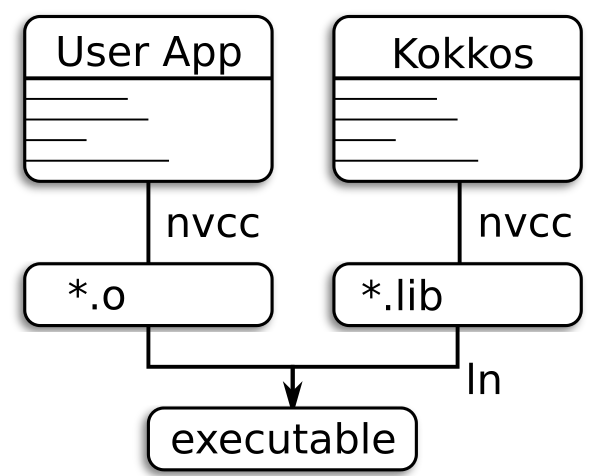
\includegraphics[width=0.3\textwidth]{img/Build.png}}
%\caption{The compilation workflow includes the invocation of the platform compiler that is in charge to generate parallel   Building workflow}
%\label{fig:workflow}  
%\end{figure}                %label: chap:example
%\section{Tutorials}\label{chap:tutorial}

The Kokkos programming model distribution~\cite{KOKKOS_REPO} includes many examples and benchmark applications as well as tutorial and presentation material. Example applications demonstrate the use of each abstraction as well supported paradigms. Examples cover the use of unified virtual memories on CUDA devices and object polymorphism in Kokkos (virtual functions). The tutorial inclemently introduces the interested reader to Kokkos abstractions and patterns. For the purpose of education each incremental step includes two code version. One code version represents the programming assignment and the other is the solution. The assignment includes instructions and marked code sections that require completion. Benchmark applications provide further insight into performance implications and allows for easy experimentation. Further resources are online\cite{KOKKOS_TUTORIAL}. They include presentation material as well as tutorials on application profiling and the Kokkos Kernels numerical library.              %label: chap:tutorial

\section{Towards Parallel Programming in C++}\label{chap:c++}
%\begin{itemize}
%\item Our contributions to parallel programming in C++. 
%\item Give an idea on direction in C++, and on our contributions.
%\item Maybe mention some of these: span, atomic\_ref, executors, kokkos\_class\_lambda (fixing this->...) etc.
%\end{itemize}
                    %label: chap:c++
\section{Related Work}\label{chap:related}

C++ increasingly supports parallel constructs. It is becoming increasingly possible to teach parallelism in C++ and relying on modern C++ compilers. However, at the time of publication, C++ does not support accelerators or many of the complexities of parallel computing related to accelerator programming. In courses that do not target accelerators, this can be a relevant option. Over the past decade, the Kokkos programming model has contributed to a number of current and near-future ISO-C++ features, including \emph{atomic\_ref}\cite{wg21_p0019}, \emph{mdspan}\cite{MDSPAN}, and executors.  In particular, the design of C++ executors, which are similar to Kokkos execution spaces, were influenced by this programming model. As the demand to extract performance from increasingly deep and increasingly asynchronous software stacks across a wide variety of domains increases, many C++ experts expect executors to become a central abstraction in any performance-oriented software stack. 
RAJA~\cite{Raja} is a C++ abstraction library with similarities to Kokkos. The important difference however is that Kokkos is descriptive, while RAJA is prescriptive. In Kokkos, the programming model determines how an application is mapped to the underlying hardware. RAJA provides functionality that exposes hardware details and relies on the developer to try different strategies to map kernels to architectures. RAJA is a viable option for class education in which the educator would like to expose students to the semantics of different programming models without exposing them to the detailed syntax of those models.
DPC++\cite{DPCPP} is a model developed by Intel\textsuperscript{\textregistered} for expressing parallelism across Intel hardware architectures. In addition to sharing a descriptive philosophy with Kokkos, it also shares parallel patterns. Unlike Kokkos however, it targets Intel architectures only and is not vendor-agnostic. A course targeting Intel architectures, DPC++ could be a valid option.

% Alpaka Dresden
% NV Thrust


                %label: chap:related
\section{Conclusion}\label{chap:conclusion}
%...
In this work we gave an introduction to the Kokkos programming model. We presented a conceptual framework consi,  presented the Kokkos parallel prgroamming model. 
Programming support for parallel progrmaming in mainstream langiages is gaining momentung
. Programming abstraction libraries such as Kokkos, Raja and others showcase this trend. Targeting a generic parallel machine representation allows to design and efficiently use 

We emphasize the importance and welcome new development and educational use of parallel programming models that align to this trend. We believe that abstracting from vendor or architecture-specific programming models not only simplifies parallel programming in science and industry but also would support educators in teaching parallel programming.
We would also like to express gratitude to educators for taking on this important role. Further materials, including a detailed description of the programming- and machine model can be found by following the reference on the Kokkos programming mode. Finally, we would like to mention that interested developers and student can reach the development team on Slack by following the invitation link as mentioned in the reference section.
             %label: chap:conclusion

\begin{thebibliography}{00}
\bibitem{KOKKOS} H. Carter Edwards and Christian R. Trott and Daniel Sunderland, 
Kokkos: Enabling manycore performance portability through polymorphic memory access patterns, Journal of Parallel and Distributed Computing, Vol. 74, p. 3202-3216, 2014
\bibitem{RAJA} Hornung, Rich, Jones, Holger, Keasler, Jeff, Neely, Rob, Pearce, Olga, Hammond, Si, Trott, Christian, Lin, Paul, Vaughan, Courtenay, Cook, Jeanine, Hoekstra, Rob, Bergen, Ben, Payne, Josh, and Womeldorff, Geoff., ASC Tri-lab Co-design Level 2 Milestone Report 2015, United States, 2015
\bibitem{NALU} Stefan Domino, Shreyas Ananthan, Robert Knaus, and Alan Williams, 
Deploy Nalu/Kokkos algorithmic infrastructure with performance benchmarking, ECP Milestone Report, United States, 2017
\bibitem{KOKKOSUSECASE1} Holmen, John K. and Humphrey, Alan and Sunderland, Daniel and Berzins, Martin, Improving Uintah’s Scalability Through the Use of Portable Kokkos-Based Data Parallel Tasks, Proceedings of the Practice and Experience in Advanced Research Computing 2017 on Sustainability, ACM, United States, 2017
\bibitem{KOKKOSUSECASE2} Stan Moore, LAMMPS KOKKOS Package: The quest for performance portable MD, LAMMPS Workshop, United States, 2019
\bibitem{OPENMP} https://www.openmp.org/specifications/
\bibitem{ERLANG} Cesarini, Francesco and Thompson, Simon, ERLANG Programming, O’Reilly Media, Inc., 2009
\bibitem{DPCPP} https://software.intel.com/en-us/oneapi/base-kit\#specifications
\bibitem{KOKKOS_REPO} https://github.com/kokkos/
\bibitem{KOKKOS_TUTORIAL} https://github.com/kokkos/kokkos-tutorials/
\bibitem{KOKKO_SLACK} https://kokkosteam.slack.com
\end{thebibliography}

\end{document}
